\documentclass[a4paper, fleqn]{article}
\usepackage[utf8]{inputenc}
\usepackage{amsmath}
\usepackage{amssymb}
\usepackage{caption}
\usepackage{mathtools}
\usepackage{amsfonts}
\usepackage{lastpage}
\usepackage{tikz}
\usepackage{float}
\usepackage{textcomp}
\usepackage{kbordermatrix}
\usetikzlibrary{patterns}
\usepackage{pdfpages}
\usepackage{gauss}
\usepackage{fancyvrb}
\usepackage[table]{colortbl}
\usepackage{fancyhdr}
\usepackage{graphicx}
\usepackage[margin=2.5 cm]{geometry}

\setlength\parindent{0pt}
\setlength\mathindent{75pt}

\definecolor{listinggray}{gray}{0.9}
\usepackage{listings}
\lstset{
	language=,
	literate=
		{æ}{{\ae}}1
		{ø}{{\o}}1
		{å}{{\aa}}1
		{Æ}{{\AE}}1
		{Ø}{{\O}}1
		{Å}{{\AA}}1,
	backgroundcolor=\color{listinggray},
	tabsize=3,
	rulecolor=,
	basicstyle=\scriptsize,
	upquote=true,
	aboveskip={0.2\baselineskip},
	columns=fixed,
	showstringspaces=false,
	extendedchars=true,
	breaklines=true,
	prebreak =\raisebox{0ex}[0ex][0ex]{\ensuremath{\hookleftarrow}},
	frame=single,
	showtabs=false,
	showspaces=false,
	showlines=true,
	showstringspaces=false,
	identifierstyle=\ttfamily,
	keywordstyle=\color[rgb]{0,0,1},
	commentstyle=\color[rgb]{0.133,0.545,0.133},
	stringstyle=\color[rgb]{0.627,0.126,0.941},
  moredelim=**[is][\color{blue}]{@}{@},
}

\lstdefinestyle{base}{
  emptylines=1,
  breaklines=true,
  basicstyle=\ttfamily\color{black},
}

\pagestyle{fancy}
\def\checkmark{\tikz\fill[scale=0.4](0,.35) -- (.25,0) -- (1,.7) -- (.25,.15) -- cycle;}
\newcommand*\circled[1]{\tikz[baseline=(char.base)]{
            \node[shape=circle,draw,inner sep=2pt] (char) {#1};}}
\newcommand*\squared[1]{%
  \tikz[baseline=(R.base)]\node[draw,rectangle,inner sep=0.5pt](R) {#1};\!}
\newcommand{\comment}[1]{%
  \text{\phantom{(#1)}} \tag{#1}}
\def\el{[\![}
\def\er{]\!]}
\def\dpip{|\!|}
\def\MeanN{\frac{1}{N}\sum^N_{n=1}}
\cfoot{Page \thepage\ of \pageref{LastPage}}
\DeclareGraphicsExtensions{.pdf,.png,.jpg}
\author{Nikolaj Dybdahl Rathcke (Student ID: 74763954)}
\title{Combinatorics \\ Assignment 1}
\lhead{Combinatorics}
\rhead{Assignment 1}

\begin{document}
\maketitle

\section*{Question 2}
We want to show $(I1)'$ is equivalent to $(I1)$ and $(I3)'$ is equivalent to $(I3)$. \\
\\
Clearly $(I1)$ implies $(I1)'$ since if $\emptyset \in \mathcal{I}$, then $\mathcal{I}\not = \emptyset$. We have that $(I1)'$ implies $(I1)$ as well, since if $\mathcal{I}\not = \emptyset$, then any $I\in \mathcal{I}$ must have the empty set as a subset.\\
Now, the condition $(I3)$ implies $(I3)'$ is easy to see as $|I_1|<|I_2|$ includes the case where $|I_2|=|I_1|+1$, so the element $e$ must exist. For the other way, we know there exists an element $e$ in $I_2-I_1$ when $|I_2|=|I_1|+1$. So no matter how large $I_2$ becomes, there will still be an element $e$ so that $I_1\cup \{e\}\in \mathcal{I}$.

\section*{Question 3}

\subsection*{Part (a)}
They do not contain the same elements as $\mathcal{I}(M_3[A])$ contains the subset $\{4,5,6\}$, but $\mathcal{I}(M_2[A])$ does not. We remember that a set of vectors are linearly independent if the matrix produced by the vectors has a non-zero determinant. Setting up the matrix $B$ produced by columns $4,5$ and $6$ gives us
\begin{align*}
  B = \begin{bmatrix}
  1 & 1 & 0 \\
  1 & 0 & 1 \\
  0 & 1 & 1
  \end{bmatrix}
\end{align*}
Calculating the determinant of $3$ by $3$ matrix can quickly be done by row reduction. Viewing it over GF(2) gives us:
\begin{align*}
    B_2 = \begin{bmatrix}
    1 & 1 & 0 \\
    1 & 0 & 1 \\
    0 & 1 & 1
    \end{bmatrix}
    \rightarrow
    \begin{bmatrix}
    1 & 1 & 0 \\
    0 & 1 & 1 \\
    0 & 1 & 1
    \end{bmatrix}
    \rightarrow
    \begin{bmatrix}
    1 & 1 & 0 \\
    0 & 1 & 1 \\
    0 & 0 & 0
    \end{bmatrix}
\end{align*}
Meaning the determinant is $0$ and the vectors are dependent. Doing the same over GF(3) gives us:
\begin{align*}
    B_3 = \begin{bmatrix}
    1 & 1 & 0 \\
    1 & 0 & 1 \\
    0 & 1 & 1
    \end{bmatrix}
    \rightarrow
    \begin{bmatrix}
    1 & 1 & 0 \\
    0 & 2 & 1 \\
    0 & 1 & 1
    \end{bmatrix}
    \rightarrow
    \begin{bmatrix}
    1 & 1 & 0 \\
    0 & 2 & 1 \\
    0 & 0 & 1
    \end{bmatrix}
\end{align*}
Giving us a determinant of $2$, non-zero, meaning the vectors are independent over this field.

\subsection*{Part (b)}
The graph the $M_2[A]$ is isomorphic to the matroid on the complete graph $K_4$.
The matroid has all subsets of size $\leq 2$, meaning the graph will be simple as it has no self-loops or parallel edges. We know the graph has $|E|=6$ edges, that it has rank $r(M)=3$ and the only dependent sets of size are $\{\{1,2,4\}, \{1,3,5\},\{2,3,6\}, \{4,5,6\}\}$. Figure \ref{fig1} shows the graph whose matroid is exactly $M_2[A]$. Let $E=\{e1, e2, e3, e4, e5, e6\}$ in the figure:
\begin{figure}[H]
  \centering
  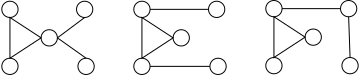
\includegraphics{fig1}
  \caption{The graph $K_4$, whose matroid is equal to $M_2[A]$}
  \label{fig1}
\end{figure}
The graph has no cycle of size $3$, any $4$ edges will contain a cycle and the only cycles of size $3$ are equal to the dependent sets mentioned above. \\
This is the only graph $G$ with $|E|=6$ and $r(M)=3$ as it must be a single connected component meaning $|V(G)|=r(M)+1=4$.  Thus, we have $M_2[A]\simeq M(K_4)$. The matroid $M_3[A]$ is not graphic as it must be isomorphic to the matroid on $K_4$, but since it contains $4$ cycles of size $3$ and $M_3[A]$ only contains $3$ dependent sets of size $3$, it cannot be graphic.

\subsection*{Part (c)}
For $M_3[A]$ to be GF(2)-representable, there must be a matrix $B$ with entries from GF(2), such that there is a one-to-one correspondence between the columns in $B$ and $E(M_3[A])$ and a set of columns are independent in $B$ iff. they are independent in $M_3[A]$. Let $f$ denote the isomorphism from $E(M_3[A])$ to $E(M_2[B])$.\\
We assume $M_3[A]$ is GF(2)-representable. That means we have that column set $\{\{1,2,4\}, \{1,3,5\}, \{2,3,6\}\}$ in $A$ are circuits, which implies that $\{\{f(1),f(2),f(4)\}, \{f(1),f(3),f(5)\}, \{f(2),f(3),f(6)\}\}$ are circuits in $M_2[A]$.


\section*{Question 4}
The circuit $C_3$ cannot be subsets of either $C_1$ or $C_2$ as one of $C_1$ and $C_2$ would not be a circuit then. This means $C_3$ cannot contain all elements in $C_1\cap C_2$ as we would be able to remove elements from $C_3$ to get either $C_1$ or $C_2$, and so $C_3=C_1$ or $C_3=C_2$. \\
This means the only possibility where $C_2-C_1\not\subseteq C_3$ or $C_3=C_1$ is when  $C_3$ is composed of the element $e$, a proper subset of $C_1\cap C_2$ and a proper subset of $C_2-C_1$. \\
Suppose $C_3$ is a circuit with the element $e$, the proper subset $I_1$ (of the intersection) and another $I_2$ (of the exclusion of $C_1$)

\section*{Question 5}
Let $M=(E,\mathcal{I})$ be the direct sum of $M_1$ and $M_2$. \\
Obviously, $(I1)$ holds for $M$ as if $\emptyset\in \mathcal{I}(M_1)$ and $\emptyset\in \mathcal{I}(M_2)$ then it also in the union set. \\
The second condition, $(I2)$, follows quite easily as well. Note that $\mathcal{I}_1$ and $\mathcal{I}_2$ are disjoint sets as $E_1$ and $E_2$ are disjoint. Thus, if $(I2)$ holds in $M_1$ and $M_2$ then it must hold in $M$, since any $I\in \mathcal{I}_1$ or $I\in \mathcal{I}_2$ will be in the union of the two. Furthermore, any $I\in \mathcal{I}_1$ cannot be a subset of an $I\in \mathcal{I}_2$ and the same the other way around. \\
Now, $(I3)$ holds as the two collections of subsets are disjoint. This means that if two sets $I_1$ and $I_2$ are from the same original matroid, then it holds as it did in $M_1$ and $M_2$. If they are from different matroids, then the set $I_2-I_1=I_2$, which means that any element $e$ we pick, it will be independent from all elements in $I_1$, and so $I_1\cup e$ will be independent.

\section*{Question 6}
Let the ground set $E=\{1,2,3\}$. Let $M_1=(E, \mathcal{I}(M_1))$ and $M_2=(E, \mathcal{I}(M_2))$ be the matroids where:
\begin{align*}
  \mathcal{I}(M_1)&=\{\emptyset, \{1\}, \{2\}, \{3\}, \{1,2\}, \{1,3\}\} \\
  \mathcal{I}(M_2)&=\{\emptyset, \{1\}, \{2\}, \{3\}, \{1,3\}, \{2,3\}\}
\end{align*}
We can see that $M_1$ and $M_2$ are indeed matroids as they satisfy $(I1),(I2)$ and $(I3)$. However, if we look at $M_3=(E, \mathcal{I}(M_3))=(E, \mathcal{I}(M_1)\cap \mathcal{I}(M_2))$, it has following collection of subsets:
\begin{align*}
  \mathcal{I}(M_3)&=\{\emptyset, \{1\}, \{2\}, \{3\}, \{1,3\}\}
\end{align*}
This is not a matroid as it does not satisfy $(I3)$. To see this, consider $I_1=\{2\}$ and $I_2=\{1,3\}$. There exists no element $e\in I_2-I_1=\{1,3\}$ such that $I_1\cup \{e\}\in \mathcal{I}(M_3)$. That is, the subsets $\{1,2\}$ and $\{2,3\}$ do not exist in $\mathcal{I}(M_3)$.

\section*{Question 7}
This is easiest shown with a counter-example. Consider the matrix:
\begin{align*}
  A=\kbordermatrix{
    & 1 & 2 & 3 \\
    & 1 & 0 & 1 \\
    & 0 & 1 & 1
  }
\end{align*}
Where $E$ is the set $\{1,2,3\}$ of column labels with the independent sets $\mathcal{I}=\{\emptyset, \{1\}, \{2\}, \{3\}, \{1,2\}, \{1,3\}. \{2,3\}\}$. Now let $\mathcal{I}^-=\mathcal{I}\cup \{1,2,3\}$. This includes the dependent subset $\{1,2,3\}$, but it still satisfies $(I1), (I2)$ and $(I3)^-$. \\
It obviously satisfy $(I1)$ and $(I2)$ as $I^-$ is the powerset of $E$, that is, all the possible subsets of $E$. Likewise, it is easy to see that the set $\mathcal{I}^-$ satisfies $(I3)^-$, since if we have two subsets $I_1$ and $I_2$ where $|I_1|<|I_2$, then you can add any element $e\in E$ (we are guaranteed there is one) to $I_1$ and that set will be in $I^-$ as it is the powerset of $E$.



\end{document}
